\documentclass[11pt]{article}
\usepackage[margin=0.8in]{geometry}
\usepackage[T1]{fontenc}
\usepackage{lmodern}
\usepackage{graphicx}
\usepackage{booktabs}
\usepackage{xcolor}
\usepackage{listings}
\usepackage{hyperref}
\usepackage{float}
\definecolor{codebg}{HTML}{F6F8FA}
\definecolor{codekw}{HTML}{2457A6}
\definecolor{codestr}{HTML}{A31515}
\definecolor{codecom}{HTML}{547547}
\lstset{language=Python,basicstyle=\ttfamily\small,backgroundcolor=\color{codebg},
  keywordstyle=\color{codekw}\bfseries,stringstyle=\color{codestr},
  commentstyle=\color{codecom}\itshape,showstringspaces=false,breaklines=true,
  frame=single,rulecolor=\color{black!18},columns=fullflexible}
\title{eBay-style Proxy Bidding with Hidden Reserve Price 60}
\author{EDSL shared-state replication note}
\date{\today}
\begin{document}
\maketitle
\begin{abstract}
This standalone report documents the sequential proxy bidding condition from the
archived llm-auction experiment. It gives the auction's shared-state machine,
the local EDSL launch path, and descriptive results from the recorded run.
The result is a new model run, not a replay of archived responses.
\end{abstract}
\section{Auction and run design}
eBay-style Proxy Bidding with Hidden Reserve Price 60. The condition uses
3 bidders, private values,
2 auction repetitions, model gpt-4,
and temperature 0.5. The archived prompts and rule template
are taken from \path{rule\_template/V10/ebay\_t4\_closing\_rule\_with\_hidden\_reserve.txt}.

\begin{table}[H]\centering\begin{tabular}{lr}\toprule
Item & Status \\\midrule
Auction condition & ebay\_reserve\_60 \\
Model & gpt-4 \\
Bidders & 3 \\
Requested auctions & 2 \\
Settled auctions & 2 \\
Completed decisions & 60 \\
Failed answers & 0 \\
State events & 123 \\
\bottomrule\end{tabular}\caption{Run coverage and state event counts.}\end{table}

\section{Shared-state machine}
Each auction repetition has an isolated scope. The machine accepts bidder actions,
exposes only its public view during play, and computes settlement in its close
transition. This prevents actions in concurrent auctions from mixing. The diagram
below was generated by the current EDSL \texttt{Machine.show\_diagram()} method.
\begin{figure}[H]\centering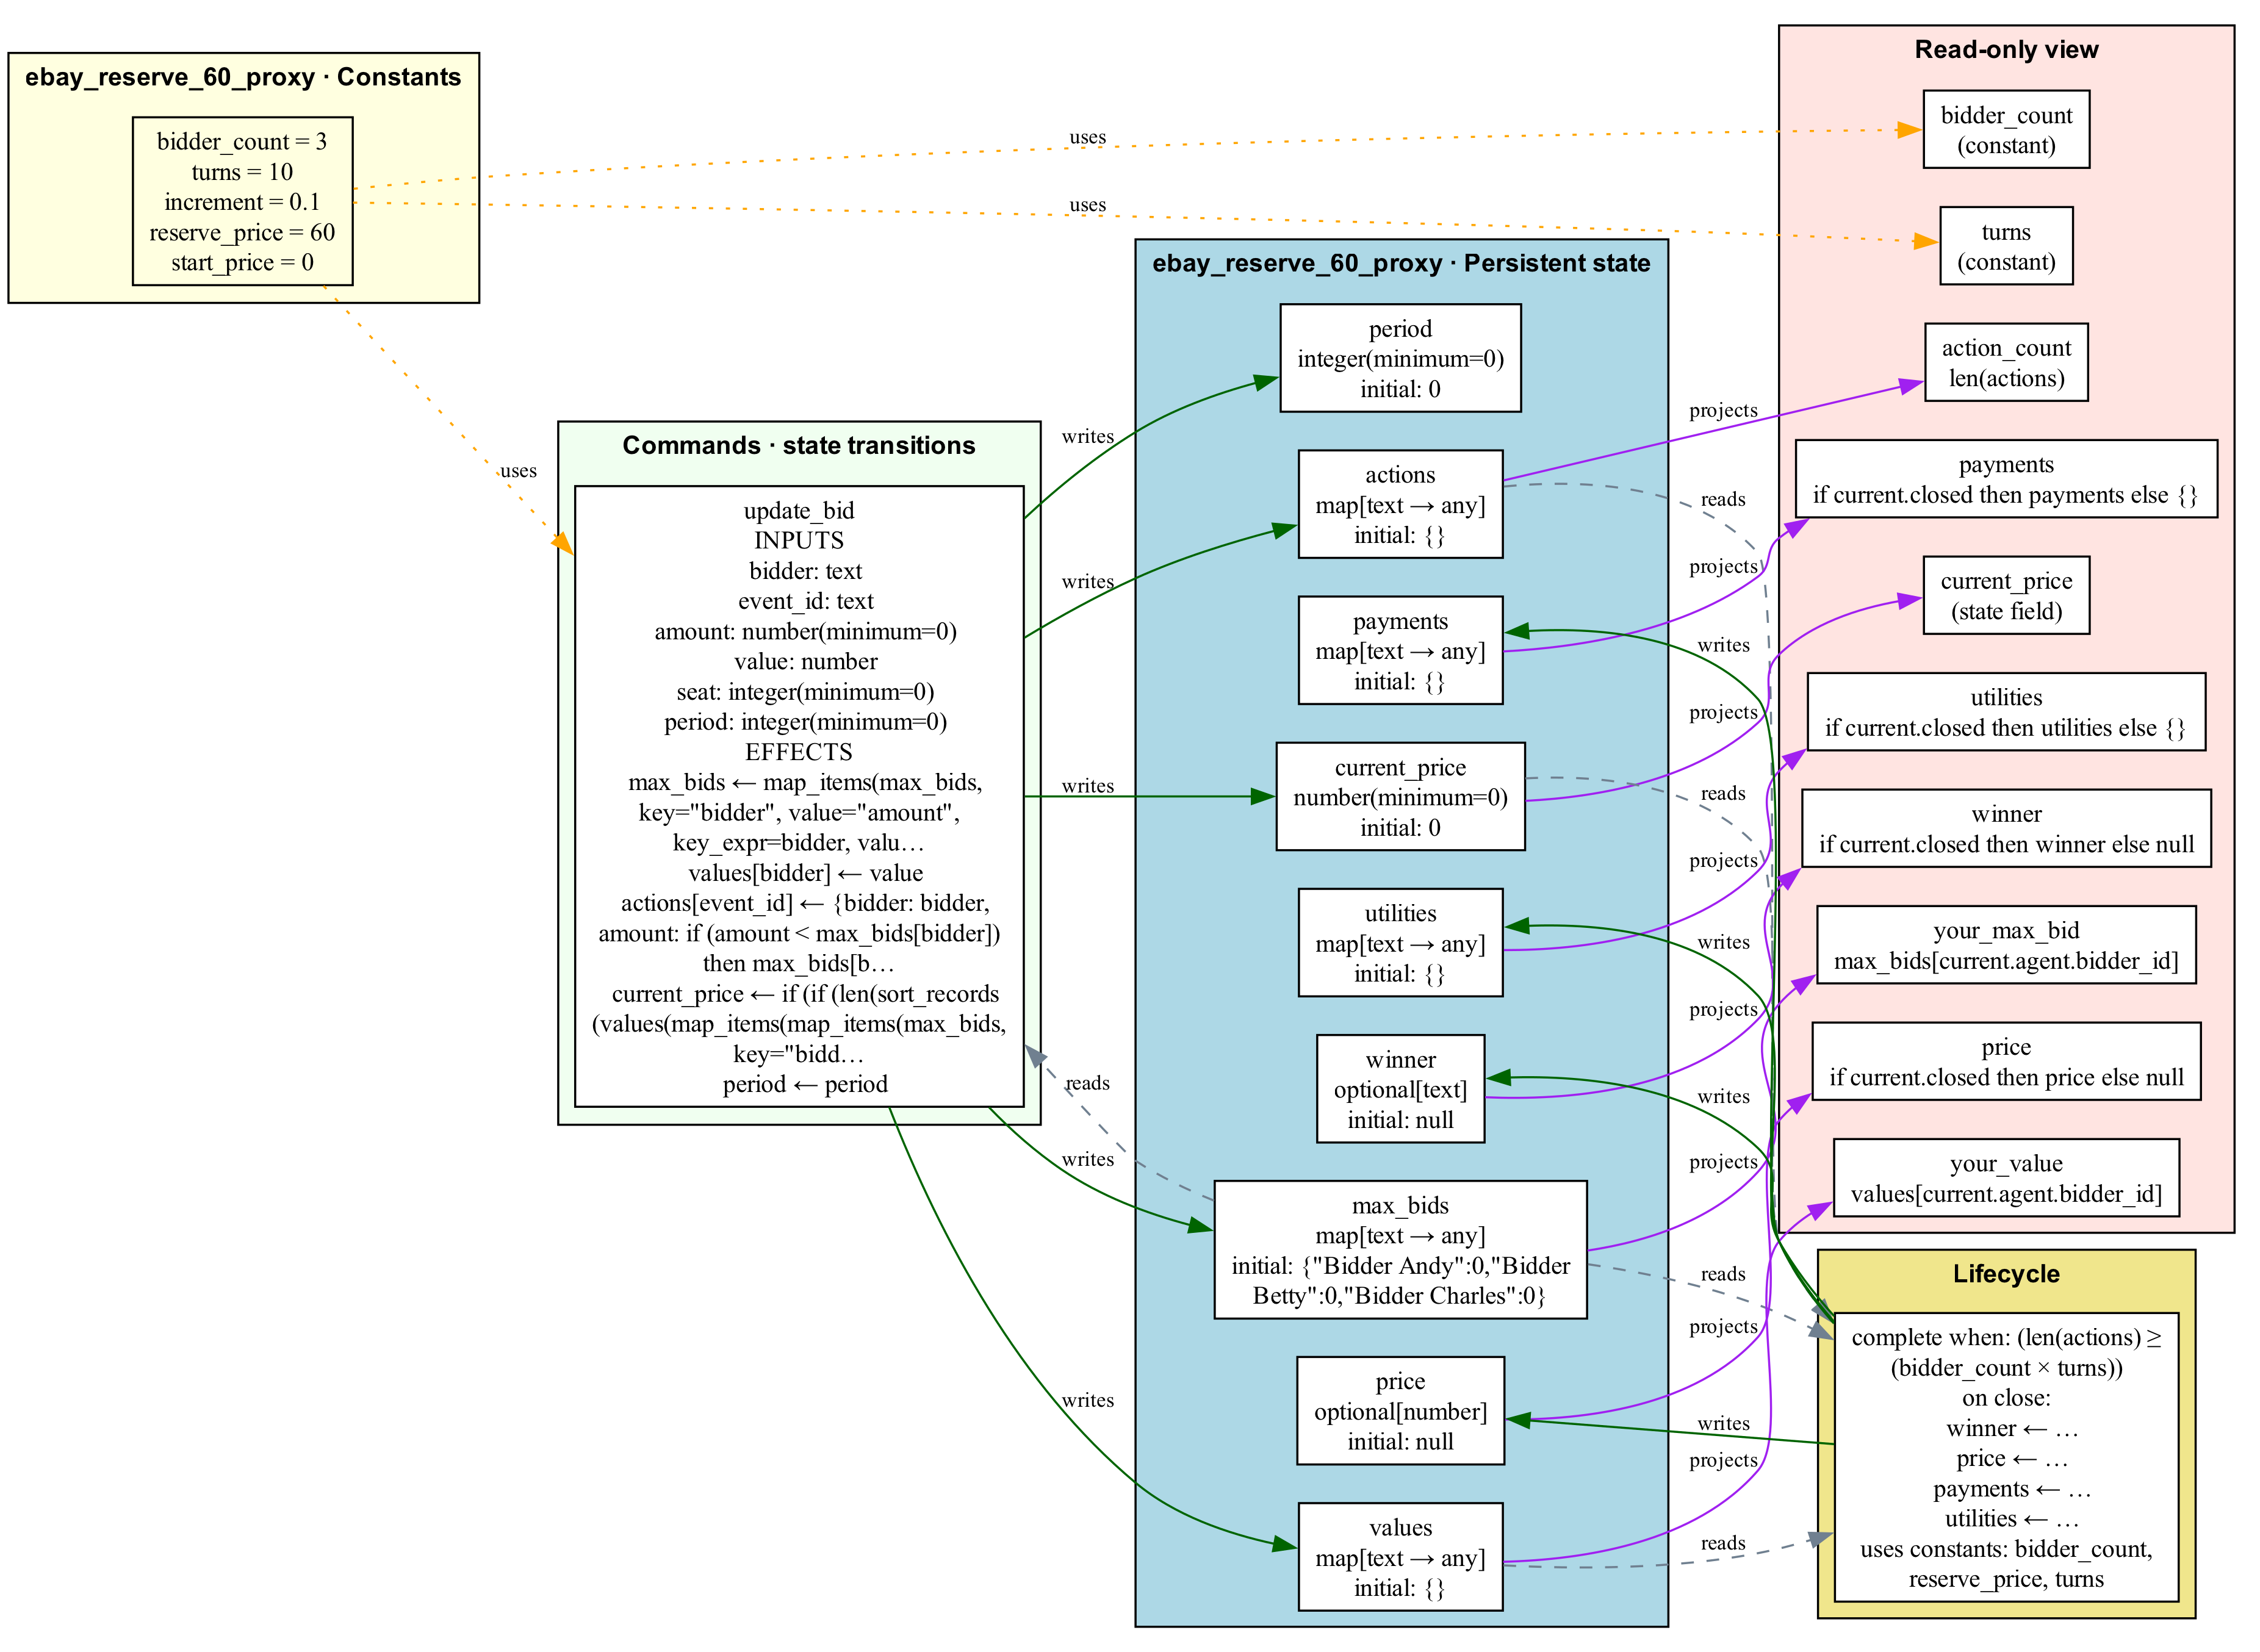
\includegraphics[width=\linewidth]{figures/state_machine.png}
\caption{State, command, view, and close lifecycle for this condition.}
\end{figure}

\subsection{Mathematical form}
Write the machine as $M=(C,X,A,V,\delta,\kappa)$, with constants $C$,
internal state $X$, action interface $A$, public view $V$, action transition
$\delta$, and close transition $\kappa$. The scope map assigns independent
states $x_r$ to auction repetitions $r$, so $\delta(x_r,a)$ cannot mutate
$x_{r'}$ when $r\ne r'$. For sealed bids, $x=(B,z)$ stores bid records
$B=\{(i,s_i,v_i,c,b_i)\}$ by bidder id; the open view reports only the
number of submissions. At close, bids are sorted by $(-b_i,s_i)$, the rule
selects rank $k\in\{1,2,3\}$ (or rank one for all-pay), and payments are
$p_i=b_i$ for every bidder in all-pay, otherwise $p_i=q$ for the winner and
zero for others. Utility is $u_i=\tilde v_i-p_i$, where $\tilde v_i$ is
the private or common component specified by the condition.

For proxy bidding, the internal state includes maximum bids $m_i$ and public
price $p$. A submitted amount $a_i$ updates $m_i\leftarrow\max(m_i,a_i)$;
if the two largest maxima are $m_1\ge m_2$, then the displayed price
is $\min(m_1,m_2+\Delta)$ when $m_2>0$, otherwise the start
price. The winner is the top maximum if the final displayed price reaches the
reserve. Each serial EDSL interview reads the latest public price before
committing its action.

\subsection{Definition used for this condition}
The implementation below is the actual Python machine factory. The archived
configuration supplies the number of bidders, payment rule, value model, reserve,
and timing constants. The close transition ranks bids by amount and stable seat,
then records payments and utilities. For proxy auctions, serial live reads expose
the updated public price while each bidder's maximum remains private.
\lstinputlisting{machine_definition.py}

\section{Local EDSL execution}
The EDSL runner executes on the local machine and calls the provider named in the
YAML using the configured API key. No localhost model server is part of this run.
The launch command for this condition is:
\begin{lstlisting}[language=bash]
python -m edsl_replication.shared_state_auctions \\
  configs/experiments/02_04_ebay_reserve_60.yaml \\
  --output edsl_replication/studies/edsl\_replication/studies/ebay\_reserve\_60/pilot\_02\_auctions/raw_results.json
\end{lstlisting}
The raw result contains the EDSL interviews, state map, machine event history, and
exit snapshots. CSV exports retain bidder-turn and auction-level observations.

\section{Observed results}
\begin{figure}[H]\centering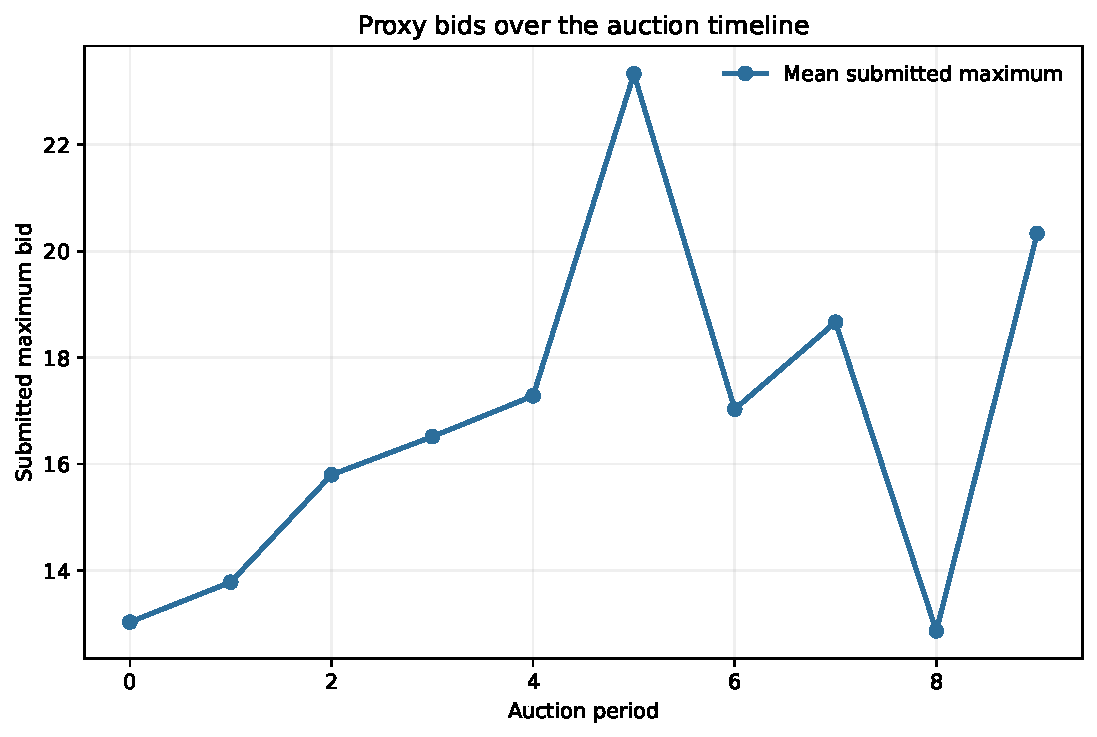
\includegraphics[width=.88\linewidth]{figures/results.pdf}
\caption{Descriptive result visualization for this condition.}
\end{figure}
\noindent Mean bidder value: 26.667; Mean bid or final maximum: 26.667; Mean bid-value gap: 0.000; Sale rate: 0.000.

The plotted pattern is descriptive. These runs use the archived prompt and
condition settings but a newly executed EDSL shared-state protocol; differences
in question structure and execution order can affect model responses.

\section{Protocol limits}
\begin{itemize}
\item Randomized within-period order is seeded; it is fixed before inference.
\item Minimum bid increment is described in prompts; numeric bids are not grid-validated.
\end{itemize}
\end{document}
